\subsection{Inversion}
In general, all inversion models implemented (e4e, ReStyle, Hyperstyle, PTI) achieve relatively good reconstruction quality as can be seen in figure \ref{fig:inversion_results}. It becomes clear that even the encoder-based method e4e can relatively well reconstruct the original images. There are however some finer details missing in the e4e inversions that the more advanced models can capture. Looking at the samples in figure \ref{fig:inversion_results}, one can see that the e4e model struggles with very fine fabric details as shown in the mesh fabric in the first and last row, and with more complex patterns as in the third and fourth row. The other methods seem to be able to capture those details, while it becomes clear that PTI seems most successful at reconstructing the dress with all details, especially the complex patterns. The results of the qualitative evaluation from figure \ref{fig:inversion_results} are also in line with the quantitative results in table \ref{tab:inversion_metrics}. Here, e4e shows the highest LPIPS and L2 scores while having the lowest MSSSIM results. Interestingly, the reconstructions show a higher FID score than the random generations obtained from the StyleGAN2-Ada model. This is also the case for ReStyle, although all other metrics show Restyle as better performing than e4e. Hyperstyle performs strictly better than both e4e and Restyle based on these metrics. This is also obvious when looking a the reconstructions in figure \ref{fig:inversion_results}. For PTI inversions, FID could not be calculated, as the model was run only for 500 dresses, which is not enough for FID calculations. The reason for the small sample size is the high inference time of 1.3 minutes per instance. The other metrics however can easily be calculated for PTI, since they are based on direct comparison of originals and reconstructions, regardless of the sample size. PTI shows superior performance in all metrics against Hyperstyle. The LPIPS score of PTI is almost half the magnitude as for Hyperstyle, indicating a considerable increase in reconstruction quality. This is also in line with the qualitative results from figure \ref{fig:inversion_results}.
\begin{figure}[ht!]
    \centering
    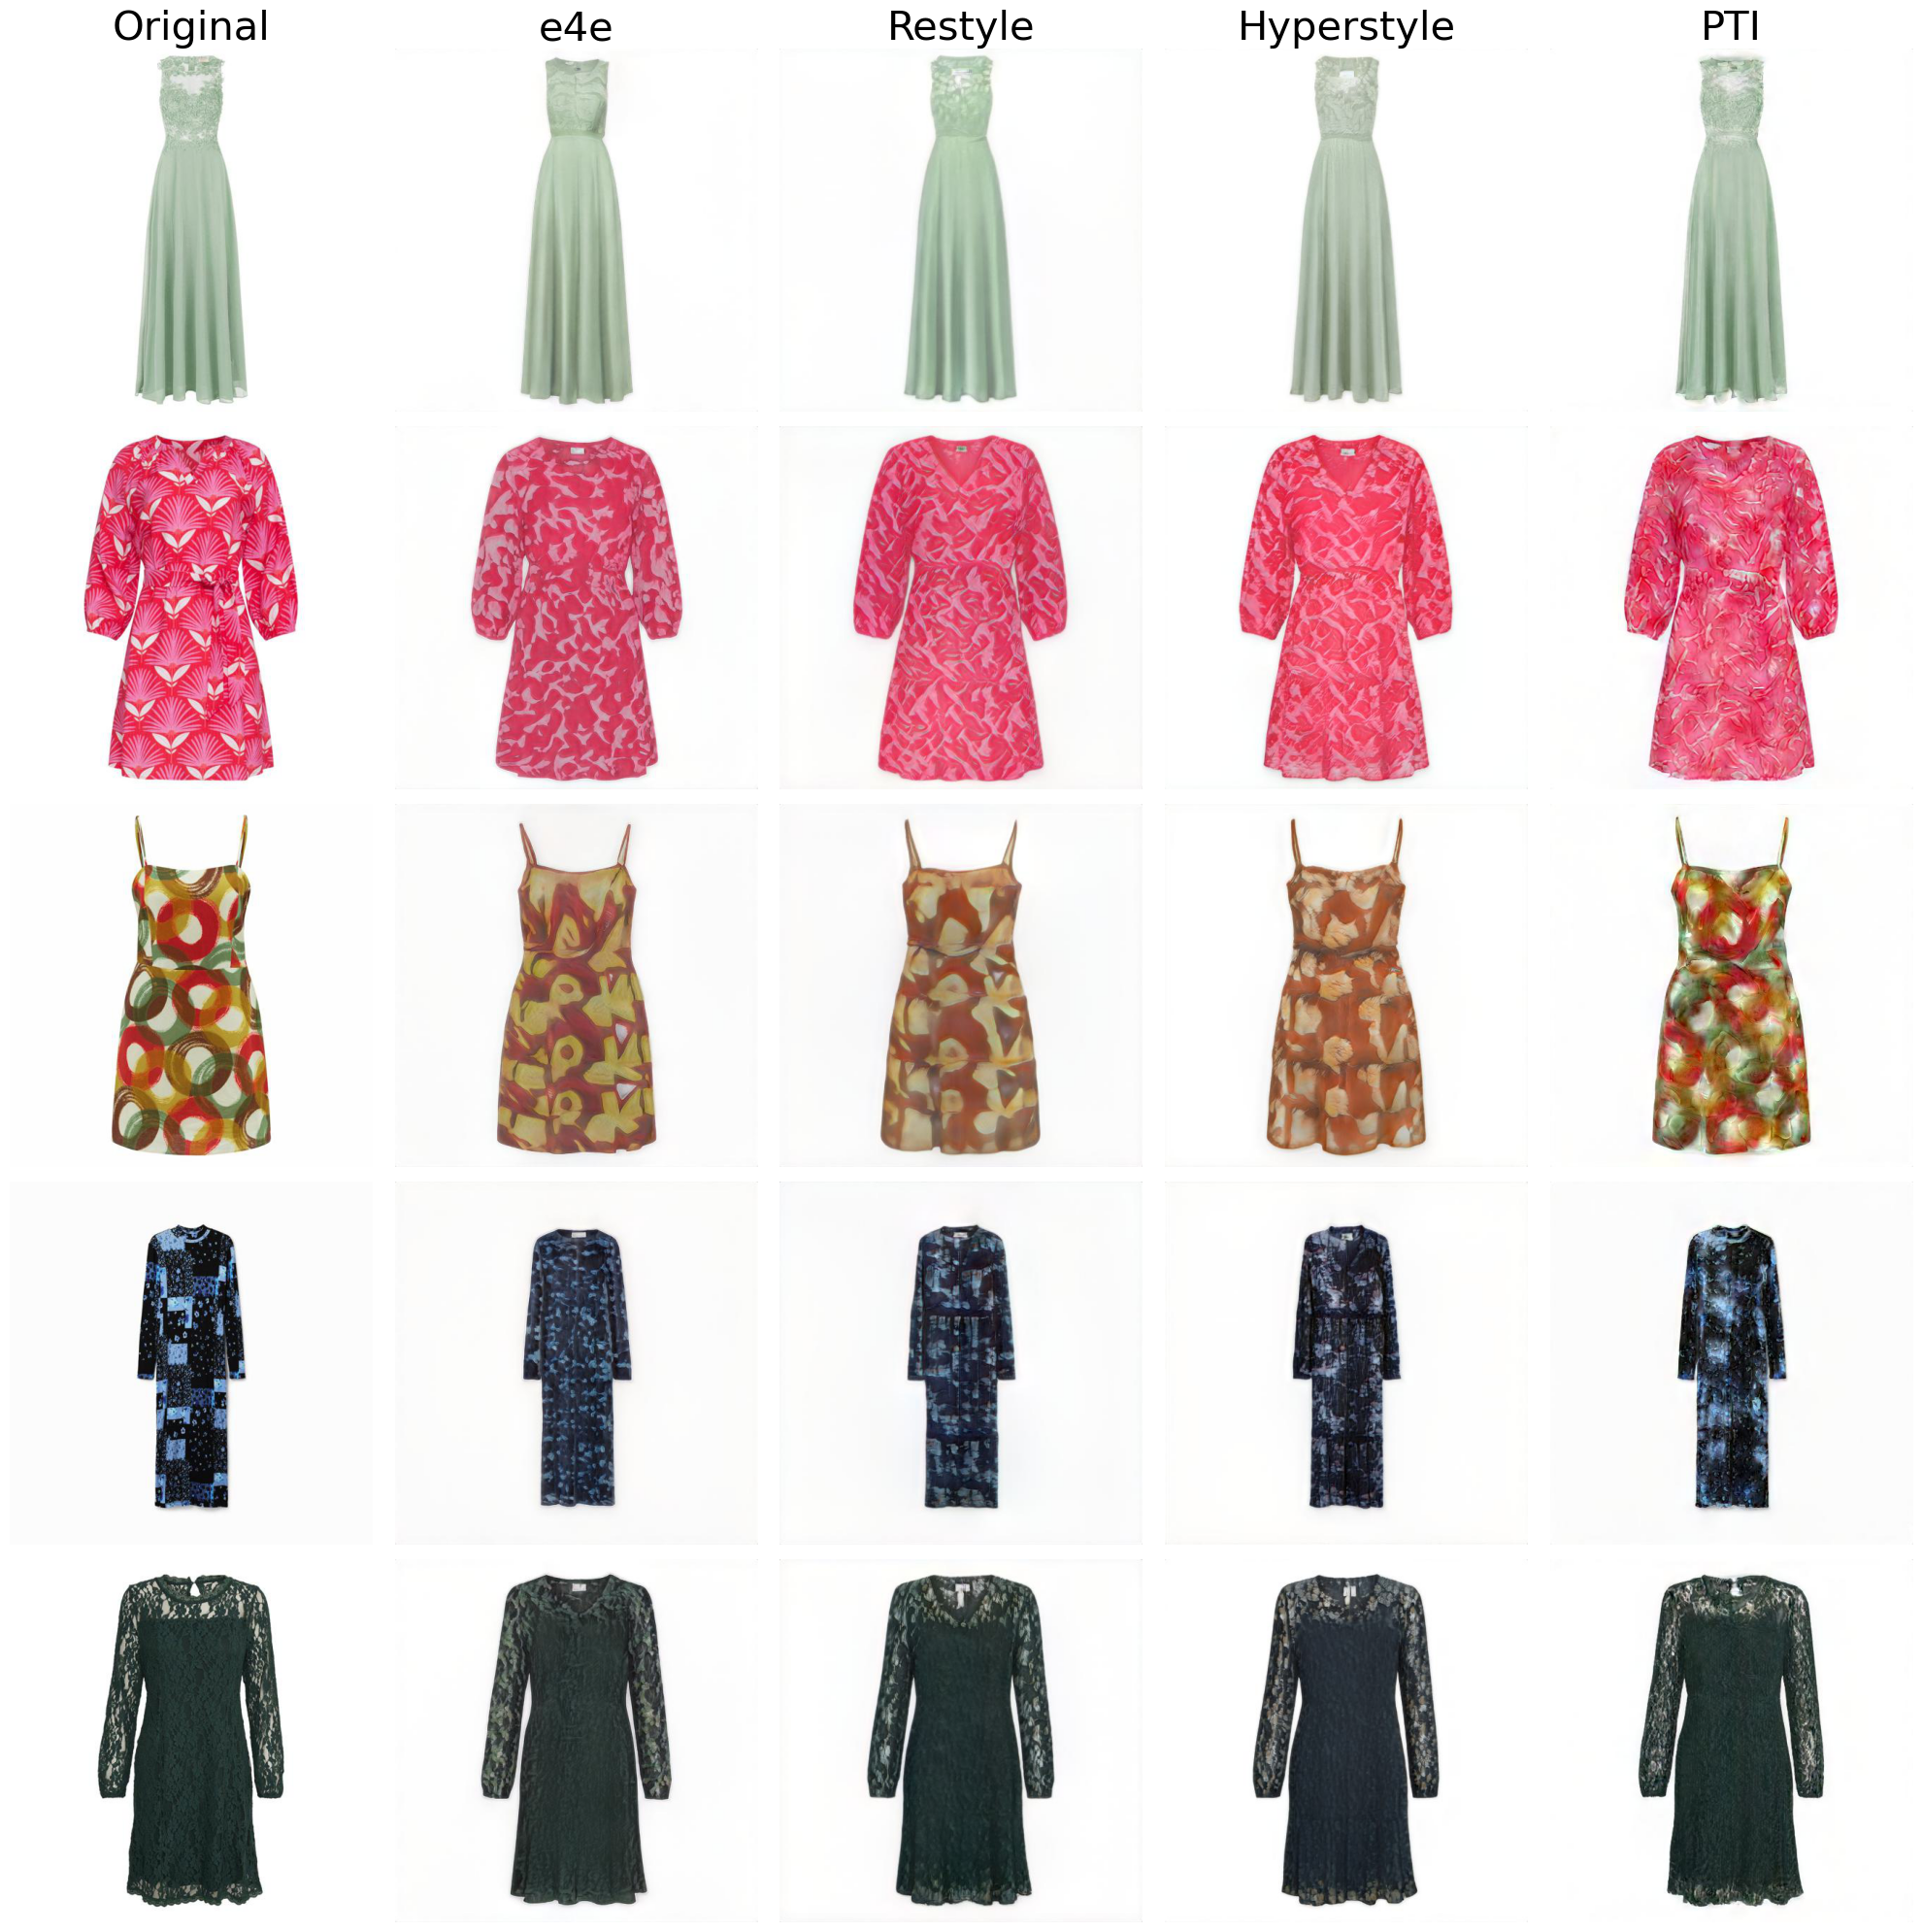
\includegraphics[width=1\linewidth]{Thesis/Results/assets/inversion_results.png}
    \caption[Qualitative Evaluation of Inversion Methods]{Qualitative Evaluation of Inversion Methods: \textit{First column shows the original image, second to last columns show the inversions obtained by various GAN-inversion methods}}
    \label{fig:inversion_results}
\end{figure}
\begin{table}[ht!]
    \centering
    \begin{tabular}{|c|c|c|c|c|c|}
        \hline
          Metric  &   StyleGAN2-Ada &       e4e &   Restyle &   Hyperstyle &    PTI \\
        \hline
        FID    &          8.0966 & 8.13   &    8.4276 &       7.1874 & -      \\
        \hline
         LPIPS  &        -      & 0.114  &    0.1138 &       0.0988 &   0.0502 \\
         \hline
         L2     &        -      & 0.0203 &    0.0147 &       0.0128 &   0.0085 \\
         \hline
         MSSSIM &        -      & 0.8702 &    0.8919 &       0.9053 &   0.945  \\
        \hline
    \end{tabular}
    \caption{Quantitative Evaluation of Inversion Methods}
    \label{tab:inversion_metrics}
\end{table}
